\section{Problem Statement}

% This section explains the problem we are solving and our motivation to do so.
Alkhidmat Foundation Pakistan, one of the largest non-profit organizations in the country, handles thousands of daily inquiries from donors, volunteers, and beneficiaries regarding donations, healthcare, and community welfare programs. Currently, these queries are managed manually through phone calls, emails, or in-person visits. This system leads to inefficiencies, delayed responses, redundant questions, and overburdened staff while also alienating overseas or low-literacy users as they struggle to navigate static website content or locate authentic project data 

The lack of an automated communication solution restricts inclusivity and accessibility, especially for marginalized communities or overseas donors seeking quick, verified information. Moreover, Alkhidmat’s operations span multiple domains; healthcare (hospitals, pharmacies, diagnostics, blood banks), education, disaster management, orphan care, women empowerment, and more, creating a vast and complex information network that manual systems cannot efficiently support. 

Hence, the problem is twofold:
\begin{enumerate}\setlength{\itemsep}{0pt}
    \item Operational burden due to repetitive, manually handled queries. 
    \item Limited accessibility for donors and beneficiaries due to language, literacy, and technology barriers. 
\end{enumerate}

The motivation behind this project is to bridge this gap by creating an AI-driven, multilingual, multimodal public chat portal that ensures inclusivity, transparency, and efficient information flow which empowers both users and staff. 

\section{Proposed Solution}

% This section gives a summary of our proposed solution, i.e. how does it solve the problem? An overview of the system is provided. A detailed description of each module of the system is presented later in Chapter ~\ref{chap:intro}.
The proposed solution is an AI-powered Public Chat Portal for Alkhidmat Foundation, a unified platform integrating a Retrieval-Augmented Generation (RAG)-based LLM with multimodal capabilities (text and image input). The portal will be accessible through Alkhidmat’s official website and WhatsApp Business API to allow seamless communication across all major user groups; donors, patients, blood donors, and beneficiaries. 

System Overview:
\begin{enumerate}\setlength{\itemsep}{0pt}
    \item \textbf{Frontend Chat Interface:} Accessible through two primary channels: 
    \begin{itemize}\setlength{\itemsep}{0pt}
        \item \textbf{WhatsApp Interface:} Integrated via the WhatsApp Business API, allowing users to chat directly through WhatsApp using text, voice notes, and image uploads. The interface employs structured message templates and quick-reply buttons for guided workflows, ensuring inclusivity for overseas donors and non-technical users. 
        \item \textbf{Web Interface:} Built in React for responsive and multilingual interaction (English, Urdu, Roman Urdu), providing a modern and intuitive experience for both desktop and mobile users. 
    \end{itemize}
    \item \textbf{Backend Services:} Powered by FastAPI and LangChain, the backend manages query classification, retrieval, and response generation. It includes: 
    \begin{itemize}\setlength{\itemsep}{0pt}
        \item \textbf{Intent Classification Module:} Determines the user’s domain of inquiry (e.g., Donation, Healthcare, Blood Services, General Support). 
        \item \textbf{Retrieval-Augmented Generation (RAG) Engine:} Combines LLM reasoning with a verified, domain-specific knowledge base to produce contextually accurate and concise responses.
        \item \textbf{Multimodal Processing Layer:} Handles image understanding and context management for smooth multimodal input handling. 
        \item \textbf{Security and Compliance Layer:} Enforces end-to-end encryption, anonymization of user data, and access control for backend APIs.
    \end{itemize}
    \item \textbf{Knowledge Base (RAG Datasets):} Curated and periodically updated datasets covering: 
    \begin{itemize}\setlength{\itemsep}{0pt}
        \item Donation and payment workflows 
        \item Healthcare and welfare program details 
        \item Donor engagement and transparency data 
        \item CSR and corporate partnership information 
        \item Accessibility and support resources 
    \end{itemize}
    \item \textbf{Human Escalation Dashboard:} A staff-facing interface where unresolved or sensitive queries are routed to human agents. Staff can respond directly, monitor conversation histories, and update relevant dataset entries. 
    \item \textbf{Analytics and Monitoring Module:} Tracks user engagement, response accuracy, and escalation frequency. Insights from these analytics help refine the system’s knowledge base and improve LLM performance over time. 
\end{enumerate}

\section{Intended User}

% This section outlines the target users of this system. The different types of users in our user base and their interaction with the system are described briefly.
The chat portal caters to three primary user groups, identified through persona analysis from workshops with Alkhidmat: 
\begin{enumerate}\setlength{\itemsep}{0pt}
    \item \textbf{Donors (Local, Overseas, Corporate):}
    \begin{itemize}\setlength{\itemsep}{0pt}
        \item Seek transparency, convenience, and verified information about donation channels, project impact, and tax compliance. 
        \item Subtypes include recurring donors, new donors, first-time donors, and CSR/corporate donors. 
    \end{itemize}
    \item \textbf{Healthcare Beneficiaries (Patients, Blood Donors, Recipients):}
    \begin{itemize}\setlength{\itemsep}{0pt}
        \item Require guidance on healthcare services, test prices, facility locations, doctor availability, ambulance booking, and Zakat-based assistance. 
        \item Includes rural and urban patients with varying digital literacy levels. 
    \end{itemize}
    \item \textbf{General Users (Public Information Seekers):} Represent individuals who approach Alkhidmat for general inquiries such as volunteer opportunities, branch contact details, upcoming drives, disaster relief information, and awareness campaigns. The chatbot provides them with general updates, project overviews, and links to participation or registration forms. 
\end{enumerate}
Through intent classification, each user’s domain (donation, healthcare, general inquiry) is automatically detected, ensuring relevant responses and routing. Administrative users (Alkhidmat staff) access a dashboard to manage escalations, update datasets, and broadcast campaigns via WhatsApp APIs. 

\section{Project gantt chart and deliverables}
% Please include a detailed gantt and details of the deliverables for Kaavish I and II
\begin{figure}[H]
    \centering
    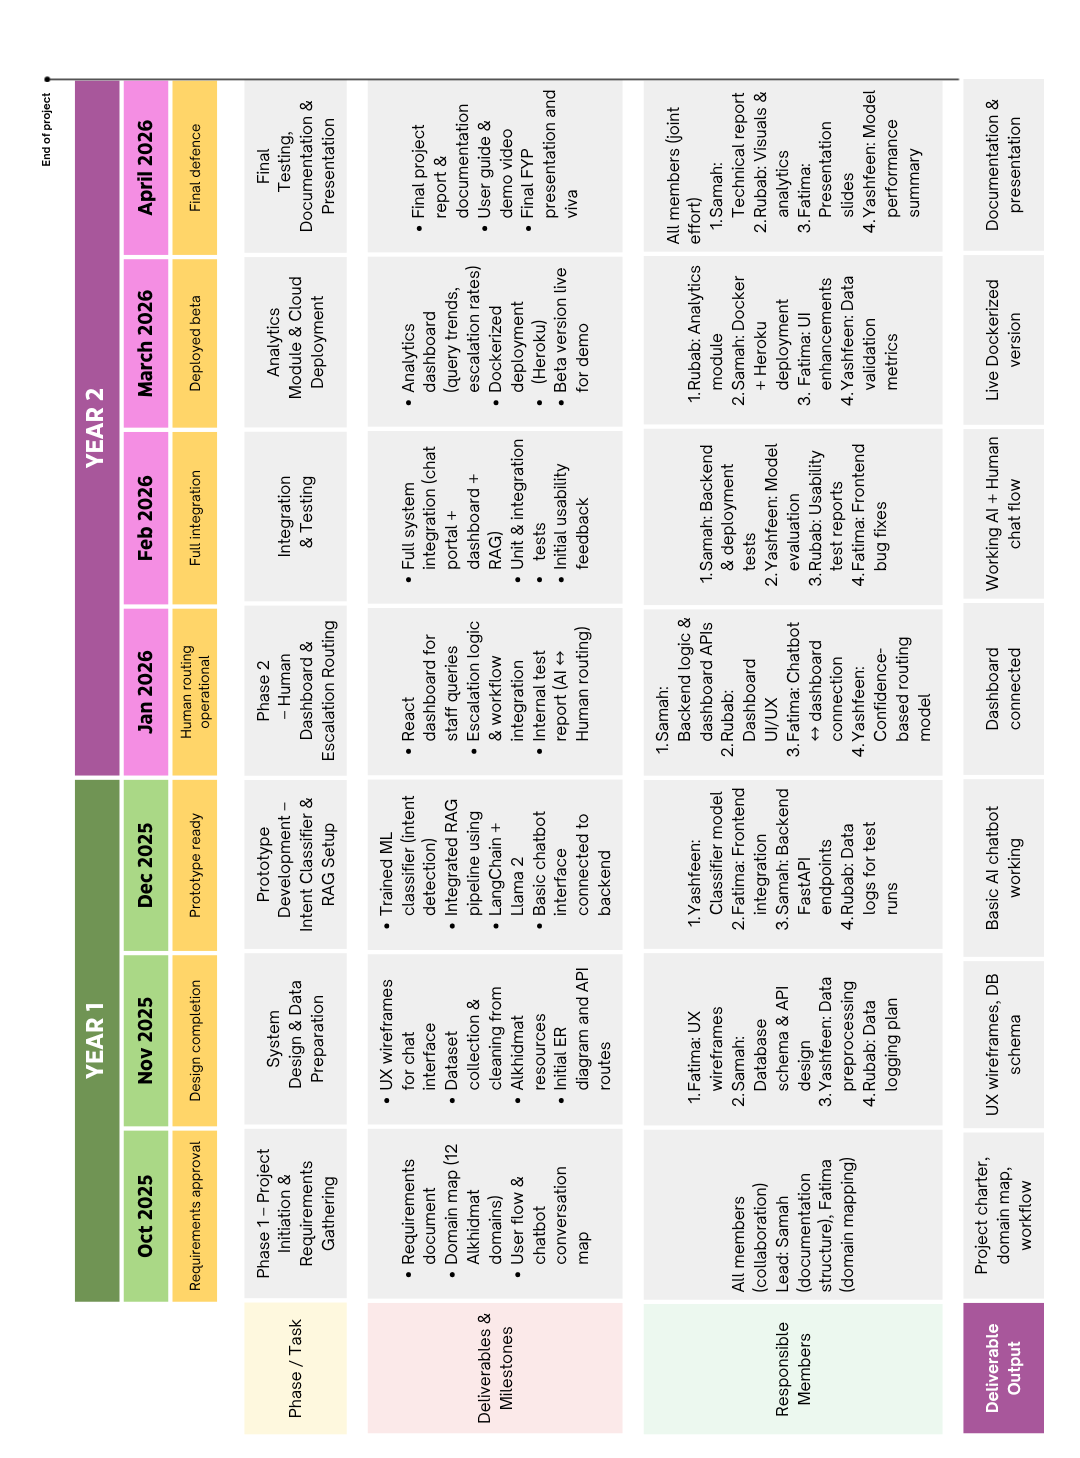
\includegraphics[width=0.8\textwidth]{chapters/GanttChart.png}
    \caption{Month-Wise Deliverables}
    \label{fig:Gantt Chart}
\end{figure}

\subsection*{Deliverables Overview}
The Gantt chart above outlines the project objectives, key milestones, and timelines for each phase across Kaavish~I and Kaavish~II. Major deliverables include:
\begin{itemize}
    \item \textbf{Kaavish I:} System requirements analysis, dataset design, RAG knowledge base creation, chatbot workflow design, and prototype implementation of the frontend and backend communication pipeline.
    \item \textbf{Kaavish II:} Integration of AI/ML modules (intent classification, multimodal processing), deployment on cloud infrastructure (Heroku/Docker), human escalation dashboard, and final evaluation with Alkhidmat’s stakeholders.
\end{itemize}

\subsection*{Resources Needed}
While the Gantt chart defines tasks, timelines, and team responsibilities, successful execution also depends on the following essential resources:

\begin{enumerate}
    \item \textbf{Hardware and Computing Resources}
    \begin{itemize}
        \item Developer laptops with minimum 16GB RAM and GPU support for model inference.
        \item Cloud hosting credits or Heroku dynos for deployment and load testing.
        \item External SSDs for backup of datasets and logs.
    \end{itemize}

    \item \textbf{Software and Development Tools}
    \begin{itemize}
        \item \textbf{Backend:} FastAPI, Python, LangChain, and Llama~2 integration.
        \item \textbf{Frontend:} React.js, Tailwind CSS, and WhatsApp Business API integration.
        \item \textbf{Database and Storage:} PostgreSQL, Elasticsearch, and Firebase (for chat logs and persona data).
        \item \textbf{Version Control and CI/CD:} GitHub, Docker, and Heroku pipelines.
    \end{itemize}

    \item \textbf{AI/ML and Data Resources}
    \begin{itemize}
        \item Access to pretrained LLMs (e.g., Llama~2 or OpenAI API for evaluation).
        \item Dataset curation support from Alkhidmat domain experts for healthcare, donation, and welfare programs.
        \item Preprocessing tools for Roman Urdu and Urdu text normalization.
    \end{itemize}

    \item \textbf{Human Resources}
    \begin{itemize}
        \item \textbf{Development Team:} 4 members (Frontend, Backend, NLP, and Integration roles).
        \item \textbf{Supervisors:} Internal advisor for technical oversight; external industry mentor from Alkhidmat.
        \item \textbf{Domain Experts:} Staff providing verified data and validating chatbot responses.
        \item \textbf{Test Users:} Donors, patients, and volunteers for pilot testing and feedback collection.
    \end{itemize}

    \item \textbf{Other Resources}
    \begin{itemize}
        \item Secure API keys for WhatsApp Business and cloud hosting.
        \item Access to Alkhidmat’s internal documentation, SOPs, and donation workflow data.
        \item Dataset annotation tools for custom tagging of healthcare and donation intents.
    \end{itemize}
\end{enumerate}

\noindent
These resources collectively ensure that each phase of development outlined in the Gantt chart is feasible and aligned with the technical and operational goals of the project.

\section{Key Challenges}

This section mentions the key challenges that we foresee in this project and possible ways to address them.
\begin{enumerate}
    \item \textbf{Data Acquisition and Knowledge Base Consolidation (Pre-deployment)}
    \begin{itemize}
        \item \textbf{Challenge:} Acquiring data and building a reliable RAG knowledge base is an immediate challenge since Al-Khidmat does not currently have a single, consolidated, structured database. This requires extensive web scraping and manual formatting of disparate documents across multiple domains, which is complicated by time constraints and the need for domain expertise.
        \item \textbf{Mitigation:} This challenge has been explicitly communicated to the external supervisor. The team has prioritized the most impactful datasets through user personas (e.g., Blood Donation SOPs). The mitigation strategy involves assigning a dedicated industry partner resource to gather and provide this essential, formatted data ASAP, aiming for the core datasets to be compiled within the next 1--2 weeks.
    \end{itemize}
    \item \textbf{Multilingual and Roman Urdu Accuracy (Natural Language Processing)}
    \begin{itemize}
        \item \textbf{Challenge:} Achieving high accuracy in Urdu and handling the inconsistency of Roman Urdu (Urdu written in English script) is difficult, as LLMs often lack high fidelity for low-resource languages and phonetic variations. This directly impacts the $\geq 90\%$ accuracy goal.
        \item \textbf{Mitigation:} Dedicate significant effort to curating the Urdu component of the RAG knowledge base. Employ custom preprocessing steps to normalize common Roman Urdu spellings before feeding them to the LLM/RAG engine.
    \end{itemize}

    \item \textbf{RAG Data Volatility and Latency (Data Management)}
    \begin{itemize}
        \item \textbf{Challenge:} Al-Khidmat's program details (e.g., active disaster relief efforts, current blood stock) change frequently. Since the system relies on a \textbf{periodically updated} knowledge base, there is a risk of providing outdated information, which compromises user trust and data integrity.
        \item \textbf{Mitigation:} Establish clear and enforced SLA for Admin updates to the RAG knowledge base (e.g., daily update requirement for time-sensitive domains like Blood Services). Use the Human Escalation Dashboard to flag and correct critical data mismatches immediately.
    \end{itemize}

    \item \textbf{Balancing Transparency and Privacy (Security and Ethics)}
    \begin{itemize}
        \item \textbf{Challenge:} Donors seek transparency about fund utilization, but the system must rigorously protect beneficiary and personal data (e.g., Zakat recipient details, patient health information) while maintaining local compliance standards.
        \item \textbf{Mitigation:} Implement stringent anonymization/pseudonymization for all data logs. Use guardrails to strictly prevent the LLM from generating or retrieving specific identifiable information in public responses.
    \end{itemize}

    \item \textbf{Human Handoff and Agent Training (Operational/UX)}
    \begin{itemize}
        \item \textbf{Challenge:} Ensuring a seamless handover from AI to a human agent without frustrating the user, particularly on WhatsApp where the 24-hour window constraint applies. Agents also need specialized training to use the Human Escalation Dashboard efficiently (diagnosing the bot's failure, not just the user's query).
        \item \textbf{Mitigation:} Focus on quick context loading and pre-filled response templates in the dashboard. Develop mandatory training modules for agents specifically on "AI Failure Diagnosis" and persona-aware communication.
    \end{itemize}
\end{enumerate}